% ============================================================================
%  Chapitre 6, partie III : Filtre de Kalman sur (gamma, b)
% ============================================================================

% ----------------------------------------------------------------------------
\section{Filtre de Kalman sur \texorpdfstring{$(\vect{\gamma}, \vect{b}_g, \vect{b}_a)$}{(gamma, bg, ba)}}
% ----------------------------------------------------------------------------

\subsection{État et dynamique}
\subsubsection{État estimé}
On estime la verticale et les deux biais : 
\[
    \vect{x}_k = \begin{pmatrix} \vect{\gamma}_k \\ \vect{b}_{g,k} \\ \vect{b}_{a,k} \end{pmatrix} \in \R^9
\]

\subsubsection{Dynamique}
\textbf{Dynamique de la verticale : }Pour la verticale, on part de $\dot{\vect{\gamma}} = -\hatx{\vect{\omega}}\vect{\gamma}$. Sur $[t_k, t_{k+1}]$, on a
\[
    \vect{\gamma}_{k+1} = \exp\bigl(-\Delta t\,\hatx{\vect{\omega}_k}\bigr)\vect{\gamma}_k
    = \exp\bigl(-\Delta t\,\hatx{\vect{z}_{g,k} - \vect{b}_{g,k} - \vect{\nu}_{g,k}}\bigr)\vect{\gamma}_k
\]
où l'exponentielle se calcule par la formule de Rodrigues. C'est une
rotation, donc elle conserve $\|\vect{\gamma}_k\| = 1$.

\textbf{Dynamique des biais : } Les deux biais suivent leur marche
aléatoire,
\[
    \vect{b}_{g,k+1} = \vect{b}_{g,k} + \vect{w}_{g,k},
    \qquad
    \vect{b}_{a,k+1} = \vect{b}_{a,k} + \vect{w}_{a,k}
\]


\begin{proposition}[La non-linéarité de la dynamique]
    La dynamique $\vect{x}_{k+1} = \mathcal{F}(\vect{x}_k, \vect{z}_{g,k})$
    n'est pas linéaire en $\vect{x}_k$.
\end{proposition}
\textbf{Démonstration : } au premier ordre en $\Delta t$,
$\exp\bigl(-\Delta t\,\hatx{\vect{\omega}}\bigr) \approx \Id - \Delta t\,\hatx{\vect{\omega}}$,
donc
\[
    \vect{\gamma}_{k+1} \approx \vect{\gamma}_k - \Delta t\,(\vect{z}_{g,k} - \vect{b}_{g,k})\wedge\vect{\gamma}_k
    = \vect{\gamma}_k - \Delta t\,\vect{z}_{g,k}\wedge\vect{\gamma}_k
    + \Delta t\,\vect{b}_{g,k}\wedge\vect{\gamma}_k
\]
On voit bien que le dernier terme est non-linéaire.
\subsection{Choix du filtre}
Compte tenu de la non-linéarité de la dynamique, on utilise dans un
premier temps un \emph{filtre de Kalman étendu} (EKF), le plus simple
à mettre en oeuvre. Il repose sur une linéarisation autour de
l'estimation courante, qui n'est valable que si l'erreur d'estimation
reste petite. Si ce n'est pas le cas, on passera à un filtre plus robuste aux non-linéarités, un \emph{CKF} ou un \emph{UKF}. Voici le \emph{filtre de Kalman étendu}.

\begin{definition}[Filtre de Kalman étendu]
    Soit une dynamique $\vect{x}_{k+1} = \mathcal{F}(\vect{x}_k, \vect{u}_k) + \vect{w}_k$, avec $\vect{w}_k$ le bruit de processus gaussien centré et de covariance $\mat{Q}_k$, observé par $\vect{y}_k = h(\vect{x}_k) + \vect{\nu}_k$, avec $\vect{\nu}_k$ le bruit de mesure, gaussien centré et de covariance $\mat{R}_k$.
    Le filtre de Kalman est composé de deux phases distinctes :

    \textbf{Prédiction : }
    \begin{align*}
        \hat{\vect{x}}_{k+1|k} &= \mathcal{F}(\hat{\vect{x}}_{k|k}, \vect{u}_k)\\
        \mat{P}_{k+1|k} &= \mat{F}_k\mat{P}_{k|k}\mat{F}_k^T + \mat{Q}_k
    \end{align*}
    \textbf{Mise à jour : }
    \begin{align*}
        \tilde{\vect{y}}_{k+1} &= \vect{y}_{k+1} - h(\hat{\vect{x}}_{k+1|k})\\
        \mat{S}_{k+1} &= \mat{H}_{k+1}\mat{P}_{k+1|k}\mat{H}_{k+1}^T + \mat{R}_{k+1}\\
        \mat{K}_{k+1} &= \mat{P}_{k+1|k}\mat{H}_{k+1}^T\mat{S}_{k+1}^{-1}\\
        \hat{\vect{x}}_{k+1|k+1} &= \hat{\vect{x}}_{k+1|k} + \mat{K}_{k+1}\tilde{\vect{y}}_{k+1}\\
        \mat{P}_{k+1|k+1} &= (\Id - \mat{K}_{k+1}\mat{H}_{k+1})\mat{P}_{k+1|k}
    \end{align*}
    où $\mat{F}_k$ est la jacobienne de la dynamique et $\mat{H}_{k+1}$ celle de la mesure :
    \[
        \mat{F}_k = \frac{\partial \mathcal{F}}{\partial \vect{x}}\Big|_{\hat{\vect{x}}_{k|k}, \vect{u}_k},
        \qquad
        \mat{H}_{k+1} = \frac{\partial h}{\partial \vect{x}}\Big|_{\hat{\vect{x}}_{k+1|k}}
    \]
\end{definition}

\subsection{Conception du filtre de Kalman}
\subsubsection{Prédiction}
On part de la dynamique 
\[
    \vect{x}_{k+1} = \mathcal{F}(\vect{x}_k, \vect{z}_{g,k}) =
    \left\{\begin{aligned}
        \vect{\gamma}_{k+1} &= \exp\bigl(-\Delta t\,\hatx{\vect{z}_{g,k} - \vect{b}_{g,k}}\bigr)\vect{\gamma}_k\\
        \vect{b}_{g,k+1} &= \vect{b}_{g,k}\\
        \vect{b}_{a,k+1} &= \vect{b}_{a,k}
    \end{aligned}\right.
\]
Il nous faut donc calculer la jacobienne, en notant
$\mat{E}_k = \exp\bigl(-\Delta t\,\hatx{\vect{z}_{g,k} - \vect{b}_{g,k}}\bigr)$ :
\begin{itemize}
    \item \textbf{Dérivée par rapport à $\vect{\gamma}_k$ : } $\vect{\gamma}_{k+1} = \mat{E}_k\vect{\gamma}_k$ est linéaire en $\vect{\gamma}_k$, donc
    \[
        \frac{\partial \vect{\gamma}_{k+1}}{\partial \vect{\gamma}_k} = \mat{E}_k
    \]
    \item \textbf{Dérivée par rapport à $\vect{b}_{g,k}$ : } au premier ordre en $\Delta t$, $\mat{E}_k \approx \Id - \Delta t\,\hatx{\vect{z}_{g,k} - \vect{b}_{g,k}}$, donc
    \[
        \vect{\gamma}_{k+1} \approx \vect{\gamma}_k - \Delta t\,\vect{z}_{g,k}\wedge\vect{\gamma}_k + \Delta t\,\vect{b}_{g,k}\wedge\vect{\gamma}_k
        = \vect{\gamma}_k - \Delta t\,\vect{z}_{g,k}\wedge\vect{\gamma}_k - \Delta t\,\hatx{\vect{\gamma}_k}\vect{b}_{g,k}
    \]
    d'où
    \[
        \frac{\partial \vect{\gamma}_{k+1}}{\partial \vect{b}_{g,k}} = -\Delta t\,\hatx{\vect{\gamma}_k}
    \]
    \item \textbf{Dérivée par rapport à $\vect{b}_{a,k}$ : } $\vect{\gamma}_{k+1}$ ne dépend pas de $\vect{b}_{a,k}$, donc
    \[
        \frac{\partial \vect{\gamma}_{k+1}}{\partial \vect{b}_{a,k}} = 0
    \]
    \item \textbf{Biais : } les deux biais sont constants dans $\mathcal{F}$, ce qui donne des blocs $\Id$ sur la diagonale et $0$ ailleurs.
\end{itemize}
Évaluée en $\hat{\vect{x}}_{k|k}$, la jacobienne est donc
\[
    \mat{F}_k = \begin{pmatrix}
        \hat{\mat{E}}_k & -\Delta t\,\hatx{\hat{\vect{\gamma}}_{k|k}} & 0\\
        0 & \Id & 0\\
        0 & 0 & \Id
    \end{pmatrix},
    \qquad
    \hat{\mat{E}}_k = \exp\bigl(-\Delta t\,\hatx{\vect{z}_{g,k} - \hat{\vect{b}}_{g,k|k}}\bigr)
\]
Il nous reste le calcul des matrices de covariance des bruits. On a notre vecteur de bruits de processus :
\[
    \vect{n}_k = \begin{pmatrix} \vect{\nu}_{g,k}\\ \vect{w}_{g,k}\\ \vect{w}_{a,k} \end{pmatrix}
\]
Ces bruits blancs rentrent dans la dynamique par la matrice $\mat{G}_k$ telle que $\vect{w}_k = \mat{G}_k\vect{n}_k$.
\begin{itemize}
    \item Au premier ordre, $\exp\bigl(-\Delta t\,\hatx{\vect{z}_{g,k} - \vect{b}_{g,k} - \vect{\nu}_{g,k}}\bigr) \approx \Id - \Delta t\,\hatx{\vect{z}_{g,k} - \vect{b}_{g,k} - \vect{\nu}_{g,k}}$, donc $\vect{\nu}_{g,k}$ rentre dans la dynamique de $\vect{\gamma}$ avec un poids $-\Delta t\,\hatx{\vect{\gamma}_k}$, comme $\vect{b}_{g,k}$.
    \item $\vect{w}_{g,k}$ et $\vect{w}_{a,k}$ rentrent directement dans la dynamique des biais, avec un poids $\Id$.
\end{itemize}
D'où
\[
    \mat{G}_k = \begin{pmatrix}
        -\Delta t\,\hatx{\hat{\vect{\gamma}}_{k|k}} & 0 & 0\\
        0 & \Id & 0\\
        0 & 0 & \Id
    \end{pmatrix}
\]
Les trois bruits sont centrés et indépendants, donc
\[
    \mat{Q}_k = \mathbb{E}\bigl[\vect{w}_k\vect{w}_k^T\bigr]
    = \mat{G}_k\,\mathbb{E}\bigl[\vect{n}_k\vect{n}_k^T\bigr]\mat{G}_k^T
    = \begin{pmatrix}
        \sigma_g^2\Delta t^2\,\hatx{\hat{\vect{\gamma}}_{k|k}}\hatx{\hat{\vect{\gamma}}_{k|k}}^T & 0 & 0\\
        0 & \sigma_{bg}^2\Delta t\,\Id & 0\\
        0 & 0 & \sigma_{ba}^2\Delta t\,\Id
    \end{pmatrix}
\]

\begin{proposition}[Linéarisation de la dynamique]
    Au premier ordre en $\Delta t$, la jacobienne de la dynamique et la covariance du bruit de processus sont
    \[
        \mat{F}_k = \begin{pmatrix}
            \mat{E}_k & -\Delta t\,\hatx{\hat{\vect{\gamma}}_{k|k}} & 0\\
            0 & \Id & 0\\
            0 & 0 & \Id
        \end{pmatrix},
        \qquad
        \mat{Q}_k = \begin{pmatrix}
            \sigma_g^2\Delta t^2\,\hatx{\hat{\vect{\gamma}}_{k|k}}\hatx{\hat{\vect{\gamma}}_{k|k}}^T & 0 & 0\\
            0 & \sigma_{bg}^2\Delta t\,\Id & 0\\
            0 & 0 & \sigma_{ba}^2\Delta t\,\Id
        \end{pmatrix}
    \]
    avec $\mat{E}_k = \exp\bigl(-\Delta t\,\hatx{\vect{z}_{g,k} - \hat{\vect{b}}_{g,k|k}}\bigr)$.
\end{proposition}

\subsubsection{Système de mesure}
\begin{remarque}[\textbf{Trade-off états-mesures}]
    Le modèle de l'accéléromètre fait intervenir $\dot{\vect{\omega}}_k$, qui n'est pas mesuré.
    On pourrait ajouter $\vect{\omega}$ et $\dot{\vect{\omega}}$ à l'état, mais il faudrait alors leur
    donner une dynamique, c'est-à-dire intégrer les équations d'Euler--Lagrange--d'Alembert dans le filtre.
    Celles-ci font intervenir l'inertie que l'on cherche à estimer et puis toutes les contraintes que l'on cherche à éviter, ce qui ne vaut pas la peine ici.
    On préfère estimer $\dot{\vect{\omega}}_k$ directement à partir du gyromètre, et faire absorber l'erreur commise par la covariance de mesure.
\end{remarque}
On estime $\dot{\vect{\omega}}_k$ par différence finie :
\[
    \hat{\dot{\vect{\omega}}}_k = \frac{\vect{z}_{g,k+1} - \vect{z}_{g,k}}{\Delta t}
\]
Le biais $\vect{b}_g$ disparaît presque dans la différence, mais le bruit est amplifié :
\[
    \hat{\dot{\vect{\omega}}}_k - \dot{\vect{\omega}}_k \approx \frac{\vect{\nu}_{g,k+1} - \vect{\nu}_{g,k}}{\Delta t},
    \qquad
    \mathbb{E}\Bigl[\bigl(\hat{\dot{\vect{\omega}}}_k - \dot{\vect{\omega}}_k\bigr)\bigl(\hat{\dot{\vect{\omega}}}_k - \dot{\vect{\omega}}_k\bigr)^T\Bigr] = \frac{1}{\Delta t^2} (\operatorname{Var}(\vect{\nu}_{g, k}) + \operatorname{Var}(\vect{\nu}_{g, k+1}) + \cdot)
    \approx \frac{2\sigma_g^2}{\Delta t^2}\Id
\]
On observe alors
\[
    \vect{z}_{a,k} = \bigl(g\,\Id + a\,\hatx{\hat{\dot{\vect{\omega}}}_k}\bigr)\vect{\gamma}_k + \vect{b}_{a,k} + \tilde{\vect{\nu}}_{a,k},
    \qquad
    \tilde{\vect{\nu}}_{a,k} = \vect{\nu}_{a,k} + a\,\hatx{\vect{\gamma}_k}\bigl(\hat{\dot{\vect{\omega}}}_k - \dot{\vect{\omega}}_k\bigr)
\]
La mesure est linéaire en $\vect{x}_k$, d'où
\[
    \mat{H}_k = \begin{pmatrix} g\,\Id + a\,\hatx{\hat{\dot{\vect{\omega}}}_k} & 0 & \Id \end{pmatrix},
    \qquad
    \mat{R}_k = \sigma_a^2\,\Id + \frac{2a^2\sigma_g^2}{\Delta t^2}\,\hatx{\hat{\vect{\gamma}}_k}\hatx{\hat{\vect{\gamma}}_k}^T
\]
On a ainsi gonflé $\mat{R}_k$ pour qu'elle absorbe l'erreur sur $\dot{\vect{\omega}}
_k$.

\begin{proposition}[Linéarisation du système de mesure]
    En estimant $\dot{\vect{\omega}}_k$ par $\hat{\dot{\vect{\omega}}}_k = (\vect{z}_{g,k+1} - \vect{z}_{g,k})/\Delta t$,
    la mesure de l'accéléromètre s'écrit
    \[
        \vect{z}_{a,k} = \mat{H}_k\vect{x}_k + \tilde{\vect{\nu}}_{a,k}
    \]
    avec
    \[
        \mat{H}_k = \begin{pmatrix} g\,\Id + a\,\hatx{\hat{\dot{\vect{\omega}}}_k} & 0 & \Id \end{pmatrix},
        \qquad
        \mat{R}_k = \mathbb{E}\bigl[\tilde{\vect{\nu}}_{a,k}\tilde{\vect{\nu}}_{a,k}^T\bigr]
        \approx \sigma_a^2\,\Id + \frac{2a^2\sigma_g^2}{\Delta t^2}\,\hatx{\hat{\vect{\gamma}}_k}\hatx{\hat{\vect{\gamma}}_k}^T
    \]
\end{proposition}

\subsubsection{Correction}
\begin{proposition}[Forme de Joseph]
    Pour tout gain $\mat{K}_{k+1}$, la covariance de l'erreur après la mise à jour
    $\hat{\vect{x}}_{k+1|k+1} = \hat{\vect{x}}_{k+1|k} + \mat{K}_{k+1}\tilde{\vect{y}}_{k+1}$ est
    \[
        \mat{P}_{k+1|k+1} = (\Id - \mat{K}_{k+1}\mat{H}_{k+1})\mat{P}_{k+1|k}(\Id - \mat{K}_{k+1}\mat{H}_{k+1})^T + \mat{K}_{k+1}\mat{R}_{k+1}\mat{K}_{k+1}^T
    \]
    Pour le gain de Kalman $\mat{K}_{k+1} = \mat{P}_{k+1|k}\mat{H}_{k+1}^T\mat{S}_{k+1}^{-1}$, elle coïncide avec $(\Id - \mat{K}_{k+1}\mat{H}_{k+1})\mat{P}_{k+1|k}$.
\end{proposition}
\textbf{Démonstration : }
\begin{itemize}
    \item \textbf{Erreur : } on note $\vect{e}_{k+1|k} = \vect{x}_{k+1} - \hat{\vect{x}}_{k+1|k}$. Comme $\tilde{\vect{y}}_{k+1} = \mat{H}_{k+1}\vect{e}_{k+1|k} + \tilde{\vect{\nu}}_{a,k+1}$,
    \[
        \vect{e}_{k+1|k+1} = (\Id - \mat{K}_{k+1}\mat{H}_{k+1})\vect{e}_{k+1|k} - \mat{K}_{k+1}\tilde{\vect{\nu}}_{a,k+1}
    \]
    \item \textbf{Covariance : } $\vect{e}_{k+1|k}$ et $\tilde{\vect{\nu}}_{a,k+1}$ sont indépendants et centrés, donc les termes croisés sont nuls et on obtient la forme de Joseph.
    \item \textbf{Gain de Kalman : } on a
    \[
        \mat{P}_{k+1|k+1} = \mat{P}_{k+1|k} - \mat{K}_{k+1}\mat{H}_{k+1}\mat{P}_{k+1|k} - \mat{P}_{k+1|k}\mat{H}_{k+1}^T\mat{K}_{k+1}^T + \mat{K}_{k+1}\mat{S}_{k+1}\mat{K}_{k+1}^T
    \]
    et $\mat{K}_{k+1}\mat{S}_{k+1}\mat{K}_{k+1}^T = \mat{P}_{k+1|k}\mat{H}_{k+1}^T\mat{S}_{k+1}^{-1}\mat{S}_{k+1}\mat{K}_{k+1}^T =\mat{P}_{k+1|k}\mat{H}_{k+1}^T\mat{K}_{k+1}^T$, donc les deux derniers termes s'annulent.
\end{itemize}
Les deux formes sont donc égales en exact, mais en arithmétique flottante, $(\Id - \mat{K}\mat{H})\mat{P}$ peut perdre la symétrie et la positivité de $\mat{P}$. La forme de Joseph est une somme de termes symétriques positifs : elle les conserve. C'est celle que l'on retient.

De plus, on n'est pas sûr que la mise-à-jour avec le gain de Kalman conserve la contrainte $\|\vect{\gamma}\| = 1$. On renormalise donc la verticale après la correction.

\begin{theoreme}[Phase de correction modifiée]
    Après la prédiction, la correction par l'accéléromètre s'écrit
    \begin{align*}
        \tilde{\vect{y}}_{k+1} &= \vect{z}_{a,k+1} - \mat{H}_{k+1}\hat{\vect{x}}_{k+1|k}\\
        \mat{S}_{k+1} &= \mat{H}_{k+1}\mat{P}_{k+1|k}\mat{H}_{k+1}^T + \mat{R}_{k+1}\\
        \mat{K}_{k+1} &= \mat{P}_{k+1|k}\mat{H}_{k+1}^T\mat{S}_{k+1}^{-1}\\
        \hat{\vect{x}}_{k+1|k+1} &= \hat{\vect{x}}_{k+1|k} + \mat{K}_{k+1}\tilde{\vect{y}}_{k+1}\\
        \hat{\vect{\gamma}}_{k+1|k+1} &\leftarrow \frac{\hat{\vect{\gamma}}_{k+1|k+1}}{\|\hat{\vect{\gamma}}_{k+1|k+1}\|}\\
        \mat{P}_{k+1|k+1} &= (\Id - \mat{K}_{k+1}\mat{H}_{k+1})\mat{P}_{k+1|k}(\Id - \mat{K}_{k+1}\mat{H}_{k+1})^T + \mat{K}_{k+1}\mat{R}_{k+1}\mat{K}_{k+1}^T
    \end{align*}
\end{theoreme}

\subsection{Performance du filtre de Kalman conçu}
\textbf{Protocole : } On simule la sphère pendant $T = 20$ s avec les conditions initiales du chapitre précédent, puis on génère les mesures des deux capteurs, montés sur la même IMU, avec des biais qui dérivent :
\begin{center}
\begin{tabular}{lcc}
    & gyromètre & accéléromètre \\
    \hline
    bruit blanc & $\sigma_g = 0{,}05$ rad/s & $\sigma_a = 0{,}5$ m/s$^2$ \\
    biais initial (écart-type) & $0{,}05$ rad/s & $0{,}3$ m/s$^2$ \\
    dérive du biais & $\sigma_{bg} = 5\cdot10^{-3}$ rad/s/$\sqrt{\text{s}}$ & $\sigma_{ba} = 7\cdot10^{-3}$ m/s$^2$/$\sqrt{\text{s}}$ \\
    fréquence & \multicolumn{2}{c}{100 Hz}
\end{tabular}
\end{center}
Le filtre est initialisé avec $\hat{\vect{\gamma}}_0 = \vect{z}_{a,0}/\|\vect{z}_{a,0}\|$ et des biais nuls. On compare l'estimation du filtre, la verticale « mesurée » $\vect{z}_a/\|\vect{z}_a\|$ et la vraie verticale.

\begin{figure}[h]
    \centering
    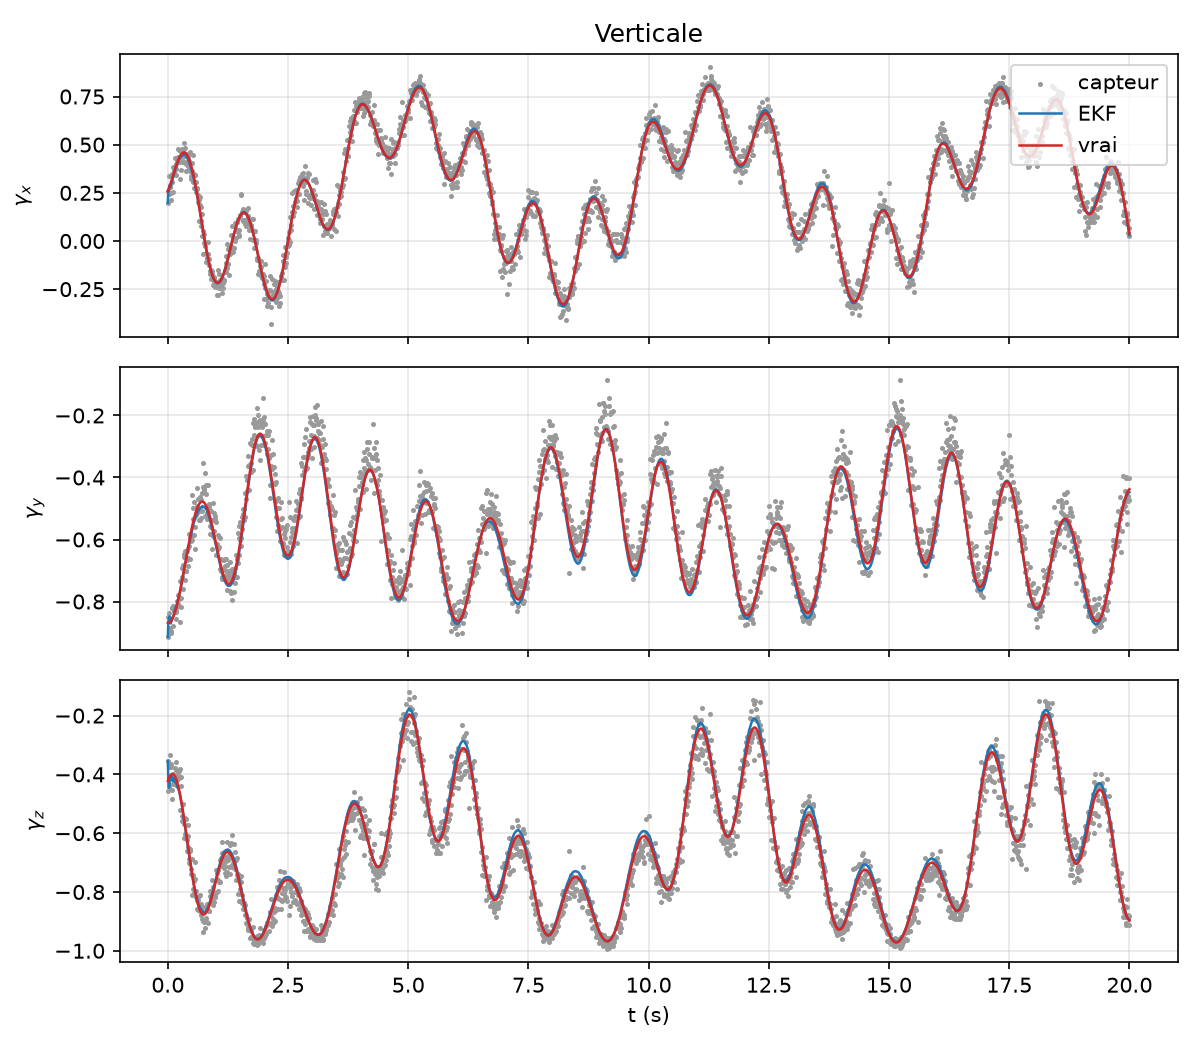
\includegraphics[width=\textwidth]{chapitre6/figures/gamma.png}
    \caption{Verticale : capteur (gris), EKF (bleu), vraie (rouge)}
    \label{fig:ekf_gamma}
\end{figure}

\textbf{Verticale : } L'erreur angulaire entre $\hat{\vect{\gamma}}$ et $\vect{\gamma}$ vaut $1{,}05^\circ$ en moyenne quadratique, contre $4{,}51^\circ$ pour l'accéléromètre seul, soit un gain d'un facteur 4. Le filtre suit la vraie verticale dès le début, sans transitoire visible.

\begin{figure}[h]
    \centering
    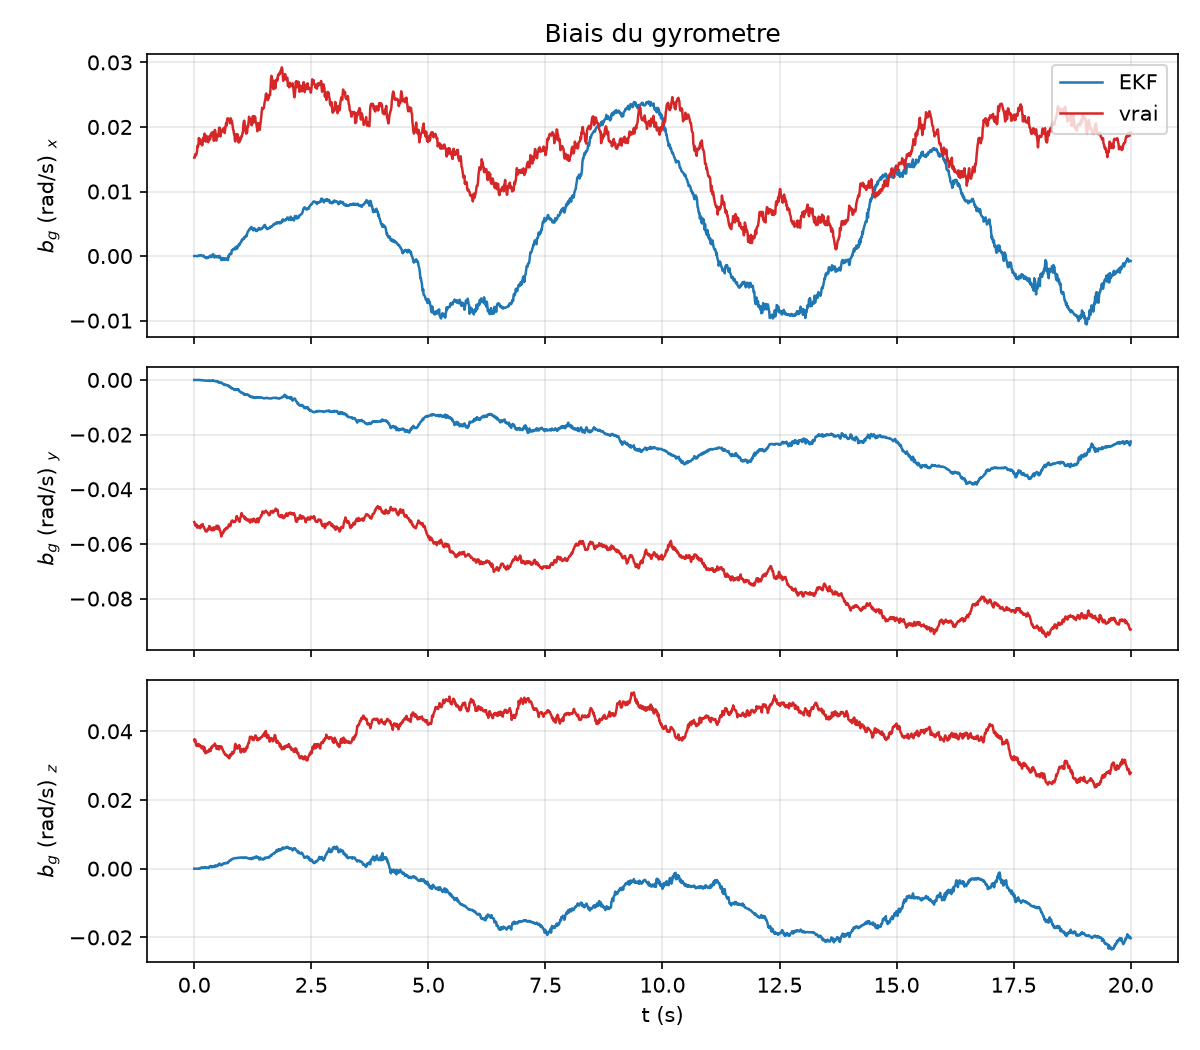
\includegraphics[width=0.49\textwidth]{chapitre6/figures/bg.png}
    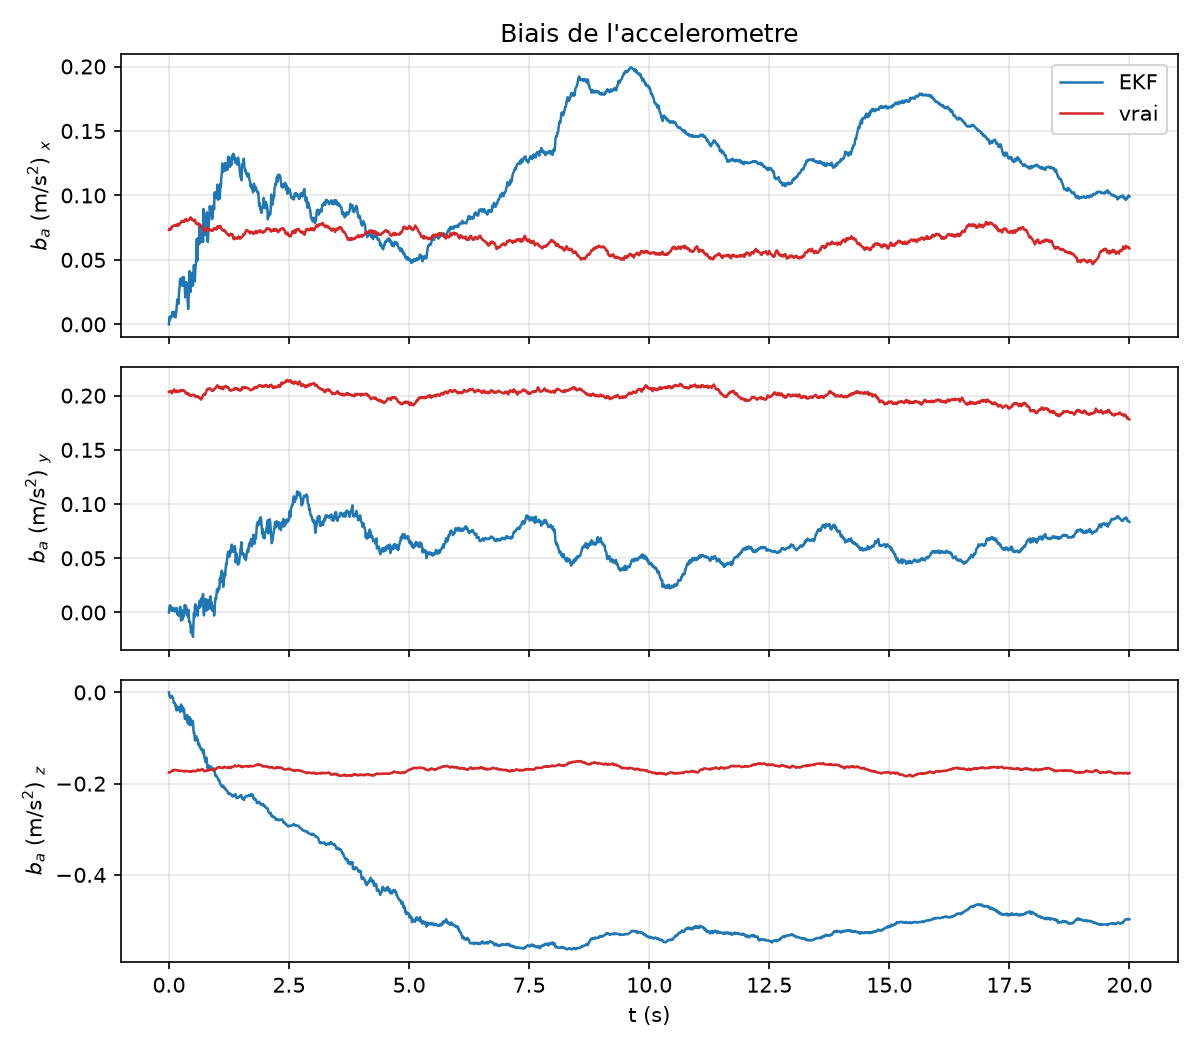
\includegraphics[width=0.49\textwidth]{chapitre6/figures/ba.png}
    \caption{Biais du gyromètre (gauche) et de l'accéléromètre (droite) : EKF (bleu), vrai (rouge)}
    \label{fig:ekf_biais}
\end{figure}
\textbf{Biais : } En revanche, les biais ne convergent pas sur 20 s.